\documentclass{beamer}

\usepackage{graphicx} % Required for inserting images

\usepackage{beamerthemesplit}

\usepackage{xmpmulti}
\usepackage{animate}
\usepackage{amsmath}
\usepackage{physics}
\usepackage{xcolor}
\usepackage{graphicx}
\usepackage{fontawesome5}
\usepackage{tcolorbox}



\usepackage{mathtools}


\usepackage{amssymb}
\usepackage{multirow}

\usepackage{physics}
\usepackage{mathrsfs}

\usepackage{tikz}
\usetikzlibrary{calc}


% \usepackage{svg}
\usepackage[inkscapeformat=png]{svg}


\usetheme{Copenhagen}
\useoutertheme{infolines}

\title[Systematic Description of W.M.]{A Systematic Description of the Wobbling Motion in Odd-Mass Nuclei Within a Semi-Classical Formalism}


% old author setup
% \author[Robert Poenaru]{%
%     \parbox[t]{0.5\textwidth}{%
%         \textbf{Author} \\
%         Robert Poenaru\inst{1} \inst{2}
%     }%
%     \parbox[t]{0.5\textwidth}{%
%         \textbf{Scientific Coordinator} \\
%         Prof. Em. Dr. A. A. Raduta\inst{2}
%     }%
% }
% \institute[DFT]{
% \inst{1} Doctoral School of Physics, UB \and %
% \inst{2} Department of Theoretical Physics, IFIN-HH
% }

% manual override for a side-by-side author view
\author[Robert Poenaru]{%
    \parbox[t]{0.45\textwidth}{%
		\centering
		\textbf{PhD Candidate} \\
		Robert Poenaru\texorpdfstring{$^{1,2}$}{(1,2)}
    }%
    \parbox[t]{0.45\textwidth}{%
		\centering
        \textbf{Scientific Supervisor} \\
        Prof. Dr. Em. A. A. Raduta\texorpdfstring{$^{2}$}{(2)}
    }%
}
\institute[IFIN-HH]{\texorpdfstring{$^{1}$}{1}Doctoral School of Physics, UB \\ \texorpdfstring{$^{2}$}{2}Department of Theoretical Physics, IFIN-HH}

\date[\today]{\textit{A presentation for the degree of Doctor of Philosophy}\vspace{0.2cm} \\ \today} % Presentation date or conference/meeting name, the optional parameter can contain a shortened version to appear on the bottom of every slide, while the required parameter value is output to the title slide



%%%%%%%%%%%%%%%%%%%%%%%%%%%%%%%%%%%%%
%%%%%%% start of the document %%%%%%%
%%%%%%%%%%%%%%%%%%%%%%%%%%%%%%%%%%%%%

\begin{document}

% trick to show a the first slide without the header
{\setbeamertemplate{headline}{}
\begin{frame}
	\titlepage % Output the title slide, automatically created using the text entered in the PRESENTATION INFORMATION block above
\end{frame}}

\begin{frame}
    \frametitle{TOC}
    \tableofcontents
\end{frame}

\section{Aim and Motivation}

\begin{frame}
    \frametitle{Aim}
    \begin{block}{\faClipboard\ Research Objectives}
        \begin{itemize}
            \item Extend the current interpretation of the \textbf{nuclear triaxiality} in the context of its unique fingerprint: \textbf{Wobbling Motion} % {\footnotesize\emph{from a theoretical standpoint}}
            \item Adopt a framework that is as close as possible to \textbf{classical physics}.
            \item Provide new formalisms for the phenomena related to \textbf{nuclear deformation}.
        \end{itemize}
    \end{block}
    \begin{exampleblock}{\faClipboard\ Objectives exclusive to the thesis}
        \begin{itemize}
            \item Give the reader enough context towards a better understanding of the underlying concepts, methods, and results.
            \item \faGithub\ create a completely \emph{open-source} project.
        \end{itemize}
    \end{exampleblock}
\end{frame}

\begin{frame}
	\frametitle{Motivation}
    \vspace{-0.3cm}
    \begin{itemize}
        \item \textbf{Nuclear Triaxiality} has become a \emph{hot topic} within the scientific community.
        \item Identifying nuclei with triaxial deformations represents a real \textbf{experimental} and \textbf{theoretical} challenge.
        % \item Experimental side: large setups, complex electronics, 
        % \item Theoretical side: cumbersome models, approximations, abstractions...
    \end{itemize}
    \vspace{-0.2cm}
    \begin{figure}
        \centering
        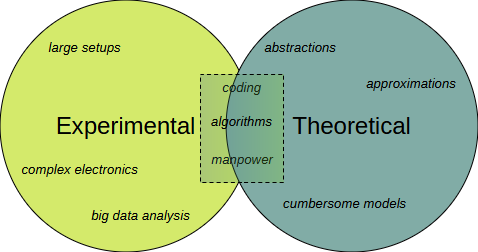
\includegraphics[width=0.85\textwidth]{figures/exp_vs_theory.png}
    \end{figure}
\end{frame}


\section{Nuclear Shapes}

\begin{frame}
	\frametitle{Nuclear Deformation}
	\begin{exampleblock}{Nuclear Radius}
		The \textbf{shape} of the nucleus is most generally described in terms of the \emph{nuclear radius}:
		\begin{align}
			R(\theta,\varphi)=R_0\left(1+\sum_{\lambda=0}^{^\infty}\sum_{\mu=-\lambda}^\lambda\alpha_{\lambda\mu}Y_\lambda^\mu(\theta,\varphi)\right)\nonumber
		\end{align}
	\end{exampleblock}
	% \begin{itemize}
	% 	\item The $\alpha_{\lambda\mu}$ are collective coordinates $\Longrightarrow$ \emph{vibrations of the nucleus}.
	% 	\item $Y_\lambda^\mu$ are the spherical harmonics.
	% \end{itemize}
	\begin{block}{Quadrupole deformations $\lambda=2$}

		\begin{itemize}
			\item {\color{red}For us:} Most relevant modes are the \textbf{quadrupole vibrations} $\lambda=2$ $\Longrightarrow$ \emph{Play a crucial role in the rotational spectra of nuclei:}
			\item \textit{Bohr, 1969}: Coordinates $\alpha_{2\mu}$ can be reduced to only two \emph{deformation parameters}: $\beta_2$ (\textbf{eccentricity}) and $\gamma$ (\textbf{triaxiality}).
		\end{itemize}
		% \begin{align}
		% 	R(\theta,\varphi)=R_0\left(1+\sum_{\mu=-2}^2\alpha_{2\mu}Y_2^\mu(\theta,\varphi)\right)\ ,
		% \end{align}
	\end{block}
\end{frame}

\begin{frame}
	\frametitle{Axial shapes}
	\vspace{-0.2cm}
	\begin{block}{Collective coordinates}
		\begin{itemize}
			\item Most of the nuclei are either \textbf{spherical} or \textbf{axially symmetric} in their ground-state \textit{(Budaca, 2018)}.
            \item Moments of inertia: $\mathcal{I}_{1,2,3}$: two are equal, one is different.
		\end{itemize}
	\end{block}
	\vspace{-0.4cm}
	\begin{figure}
		\centering
		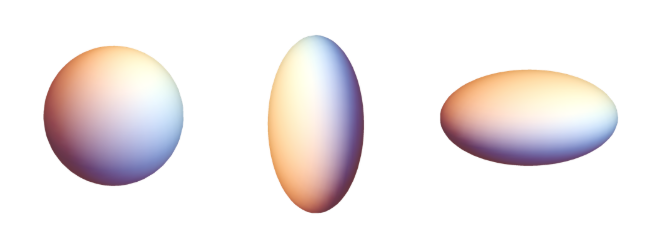
\includegraphics[scale=0.38]{figures/nuclear_shapes.png}
		\caption{\textbf{spherical:} $\beta_2=0$\ \textbf{prolate:} $\beta_2>0$\ \textbf{oblate:} $\beta_2<0$.\ ($\gamma=0^\circ$).}
	\end{figure}
\end{frame}

\begin{frame}
	\frametitle{Non-axial shapes}
	\vspace{-0.2cm}
	\begin{itemize}
		\item The triaxiality parameter $\gamma\neq 0^\circ$: departure from axial symmetry.
		\item Moments of inertia: $\mathcal{I}_{1}\neq\mathcal{I}_{2}\neq\mathcal{I}_{3}$.
	\end{itemize}
	\vspace{-0.2cm}
	\begin{figure}
		\centering
		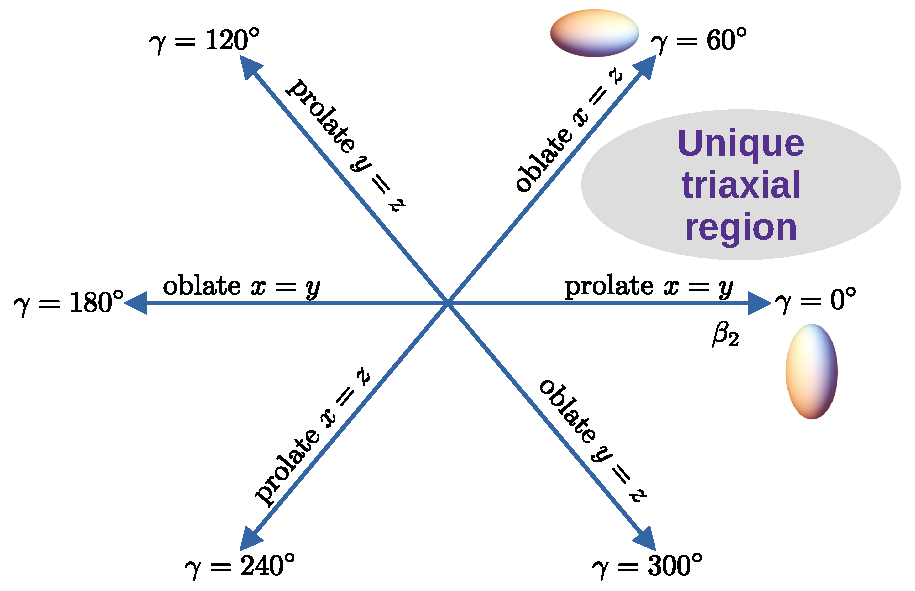
\includegraphics[scale=0.49]{figures/nice_diagram.pdf}
		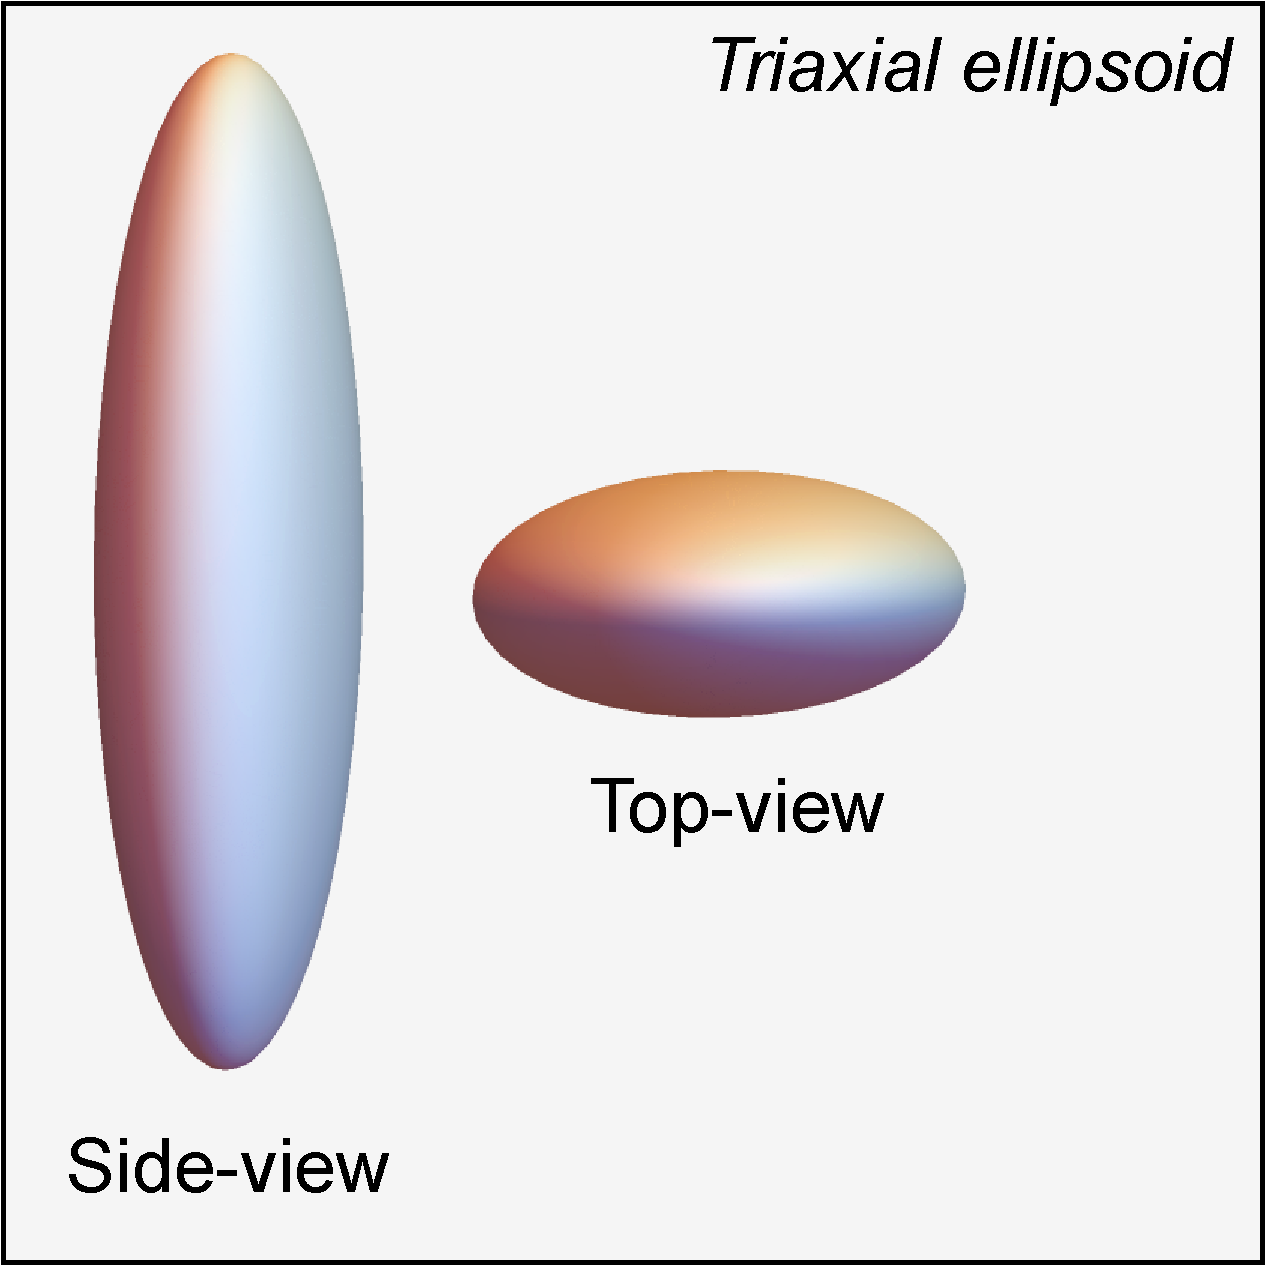
\includegraphics[scale=0.20]{figures/triaxial-shape.pdf}
		\vspace{-0.41cm}
	\end{figure}
\end{frame}

\section{Triaxiality and Wobbling Motion}

\begin{frame}
	\frametitle{Fingerprints of Triaxiality}
	\begin{block}{Evidence \faSearch}
		\begin{itemize}
			\item Currently, there are \textbf{only two} well-established phenomena uniquely attributed to triaxial deformation.
			\begin{enumerate}
				\item \textbf{Wobbling Motion} - WM (\emph{Bohr and Mottelson, 1970s})
				\item Chiral Motion - $\chi$M (\emph{Frauendorf, 1997})
			\end{enumerate}
			\item These two can be measured/detected experimentally.
		\end{itemize}
	\end{block}
	\begin{exampleblock}{\textbf{Goal} \faClipboard}
		\textbf{Describe the elusive character of Wobbling Motion in the context of nuclear triaxiality.}
	\end{exampleblock}
\end{frame}

\begin{frame}
	\frametitle{\faSearch\ Probing triaxiality in nuclei}
    Triaxial nuclei can be observed/obtained in several experiments:
    \begin{itemize}
        \item Nuclear fission: $A\ \rightarrow\ B\ +\ C$
        \item Nuclear fusion: $X\ +\ Y\ \rightarrow\ Z$
        \item \textbf{Fusion-evaporation reactions}: {\color{red}Long-lived} + {\color{red}enhanced deformation}
        \vspace{-0.3cm}
        \begin{align}
            {\color{blue}Beam(N_1,E)}\ +\ {\color{magenta}Target(N_2)}\longrightarrow N_3^*\rightarrow\dots\rightarrow {\color{purple}triaxial(N_4)} \nonumber
        \end{align}
    \end{itemize}
	\vspace{-0.3cm}
    \begin{figure}
        \centering
        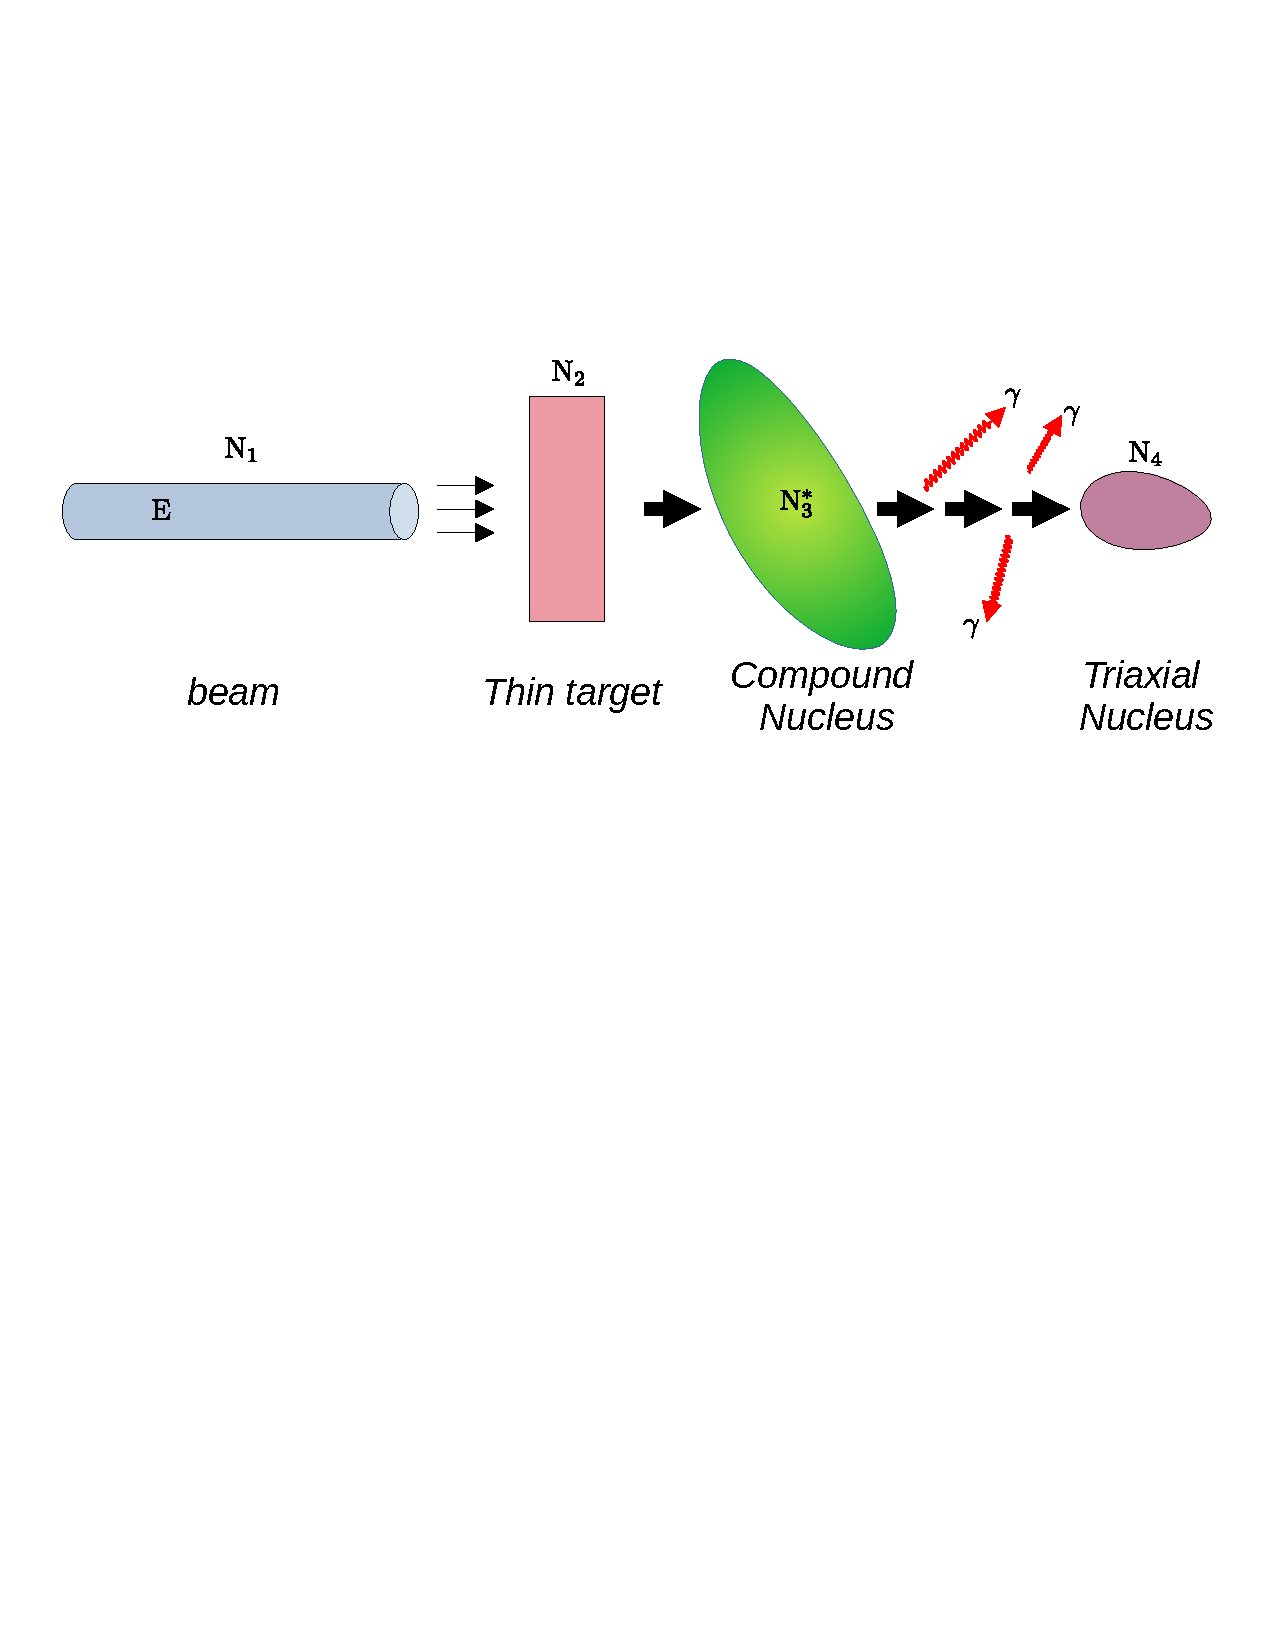
\includegraphics[width=0.99\textwidth]{figures/fusion-evaporation.pdf}
    \end{figure}
\end{frame}

\begin{frame}
	\frametitle{\faSearch\ Nuclear facilities}
	\vspace{-0.3cm}
	\begin{columns}
		\column{0.4\textwidth}
		\begin{figure}
		\centering
		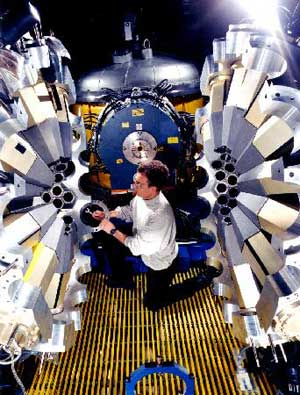
\includegraphics[width=0.88\textwidth]{figures/gsfig.jpg}
		\caption{Gammasphere detector, ANL-ATLAS USA. \textit{Source: aps.org}}
	\end{figure}
	\column{0.6\textwidth}
	\begin{figure}
		\centering
		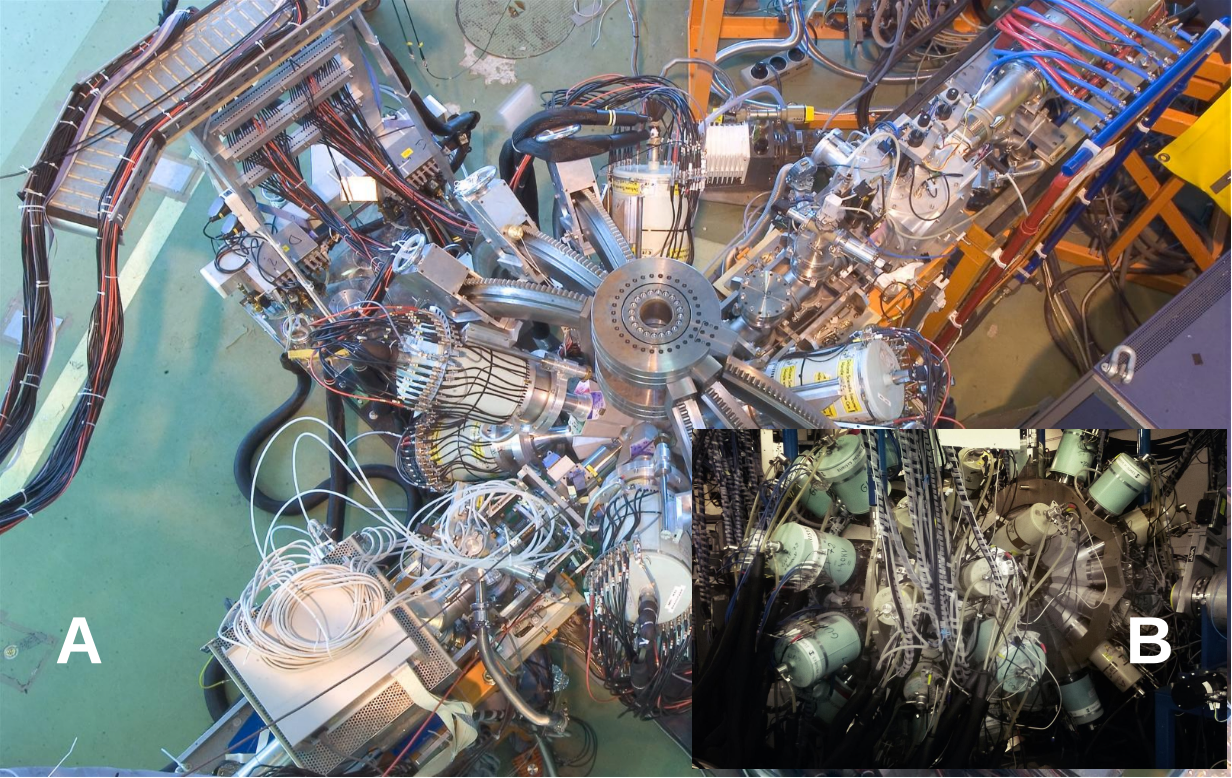
\includegraphics[width=0.99\textwidth]{figures/isolde_cern_2.png}
		\caption{a) IDS detector, CERN. \textit{Source: isolde.web.cern.ch} b) JUROGAM II, Finland. \textit{Source: twitter.com}}
		\end{figure}
	\end{columns}
\end{frame}


\begin{frame}
	\frametitle{Wobbling Motion}
	\vspace{-0.4cm}
	\begin{columns}
		\begin{column}{0.55\textwidth}
			\begin{center}
				\begin{tikzpicture}[node distance=1.5cm]
					\node[draw, fill=blue!20!white, text width=3cm, text centered, minimum height=1cm] (box1) {$\gamma\neq0^\circ$};
					\node[draw, fill=blue!20!white, text width=4cm, text centered, minimum height=1cm, below of=box1] (box2) {MOI anisotropy};
					\node[draw, fill=blue!20!white, text width=6cm, text centered, minimum height=1cm, below of=box2] (box3) {\emph{main rotation} around $\mathcal{J}_\text{max}$ is disturbed by the other two axes};
					\draw[->] (box1) -- (box2);
					\draw[->] (box2) -- (box3);
				\end{tikzpicture}
			\end{center}
		\end{column}
		\begin{column}{0.45\textwidth}
			\begin{figure}
				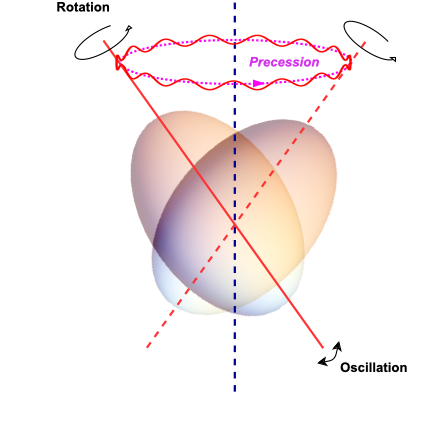
\includegraphics[width=\textwidth]{figures/wobbling-schematic.png}
			\end{figure}
		\end{column}
	\end{columns}
	\vspace{-0.4cm}
	\begin{alertblock}{Wobbling Effect}
		\begin{itemize}
			\item The \textbf{total angular momentum} of the nucleus \textbf{precesses} and \textbf{oscillates} around $\mathcal{J}_\text{max}$.
		\end{itemize}
	\end{alertblock}
\end{frame}

\begin{frame}
	\frametitle{Wobbling Motion}
	\begin{exampleblock}{Harmonic oscillation}
		\begin{itemize}
			\item Precession of $\mathbf{I}$ is affected by \textbf{rotational frequency} and/or \textbf{tilting}
			\item Tilting only by "specific" amount $\rightarrow$ \textbf{harmonic character} $\rightarrow$ \textbf{wobbling phonon}: $n_w=0,1,2,\dots$.
		\end{itemize}
	\end{exampleblock}
	\begin{figure}
		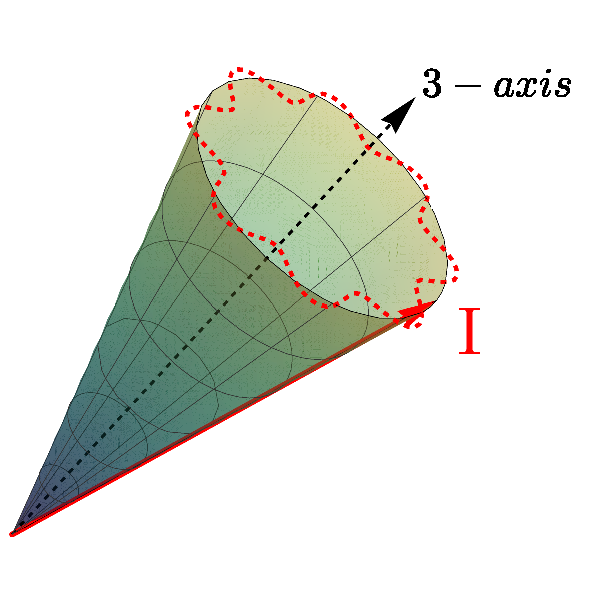
\includegraphics[width=0.32\textwidth]{figures/precessional_cone_2.pdf}
		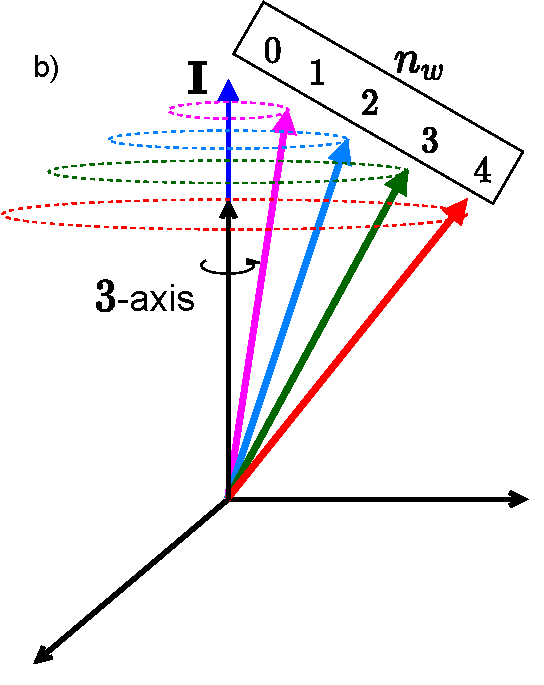
\includegraphics[width=0.3\textwidth]{figures/wobbling_n_schematic-2.pdf}
		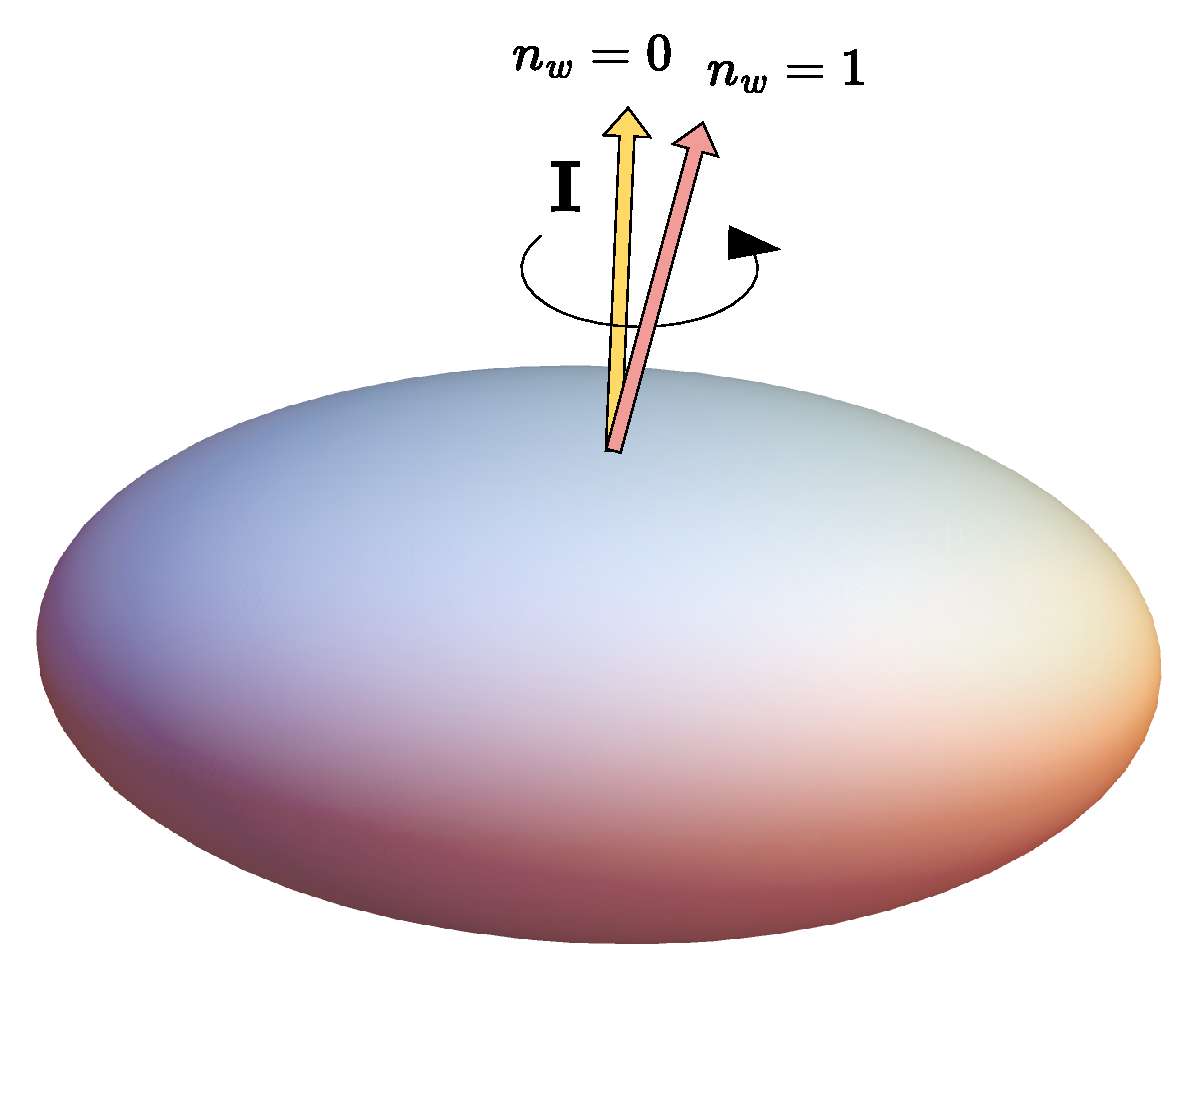
\includegraphics[width=0.34\textwidth]{figures/triaxial-shapes-even-A.pdf}
	\end{figure}
\end{frame}

\begin{frame}
	\frametitle{Wobbling Motion II}
	\vspace{-0.4cm}
	\begin{columns}
		\begin{column}{0.6\textwidth}
			\begin{figure}
				\centering
				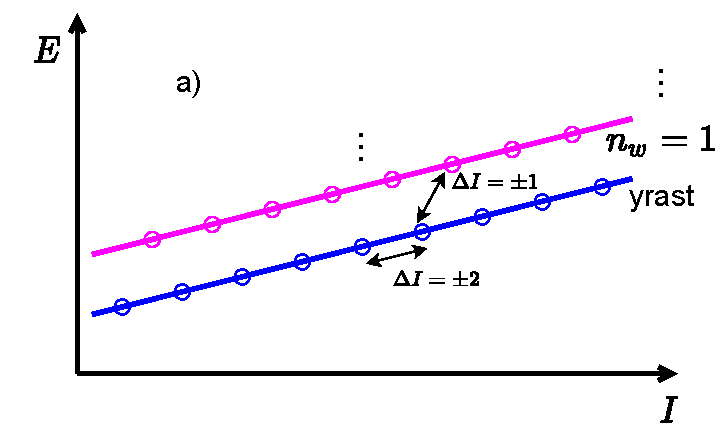
\includegraphics[scale=0.45]{figures/wobbling_n_schematic-1.pdf}
				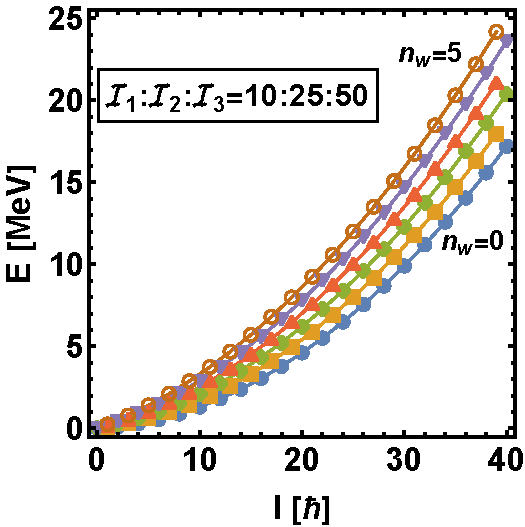
\includegraphics[scale=0.48]{figures/wobblingFreq-evenA.pdf}
			\end{figure}
		\end{column}
		\begin{column}{0.4\textwidth}
			\begin{figure}
				\centering
				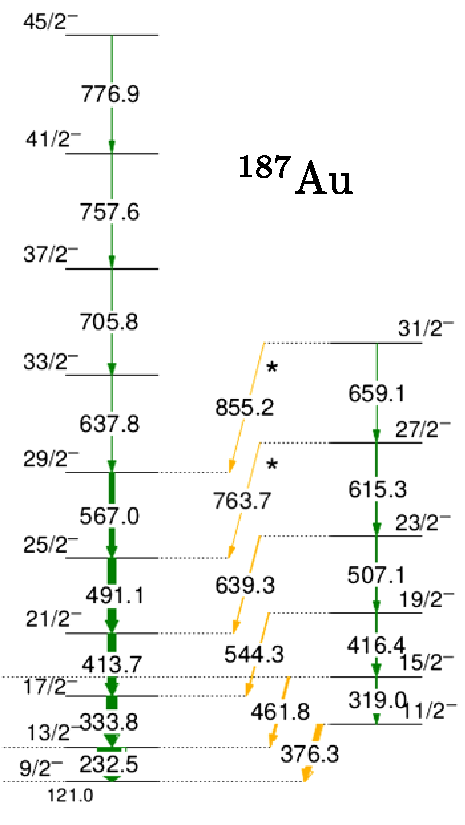
\includegraphics[width=0.8\textwidth]{figures/au_187_spectra.pdf}
			\end{figure}
			\vspace{-0.4cm}
			\textit{Sensharma, 2020}.
		\end{column}
	\end{columns}
\end{frame}

\begin{frame}
	\frametitle{Even-$A$ vs. Odd-$A$ Picture}
	\begin{itemize}
		\item Predicted for even-$A$ nuclei more than 50 years ago.
		\item First experimental evidence for \textbf{nuclear wobbling motion}: $^{163}$Lu (\textit{Ødegård, 2001}).
		\item Current mass-regions for wobblers: $A=130,160,180$.
	\end{itemize}
	\begin{figure}
		\centering
		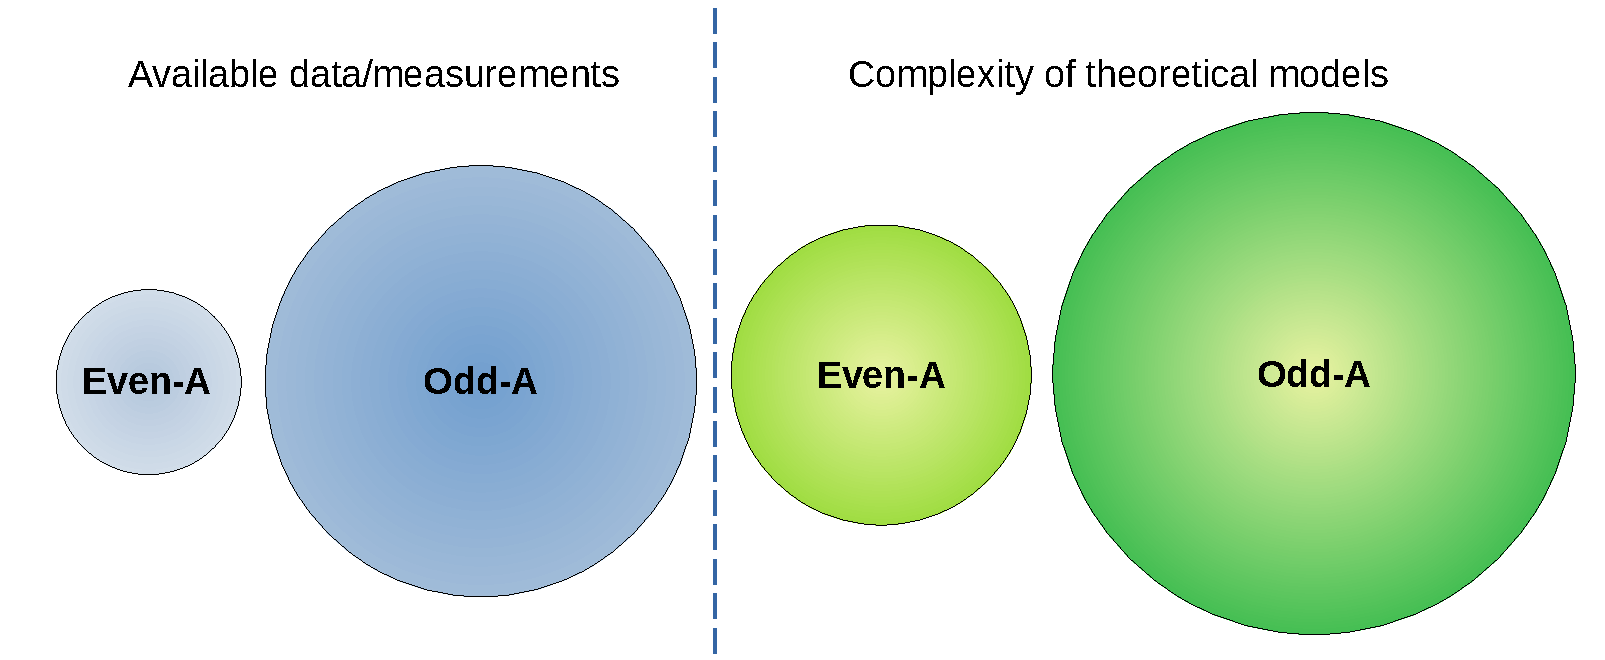
\includegraphics[width=0.99\textwidth]{figures/even-vs-odda.pdf}
	\end{figure}
\end{frame}

\begin{frame}
	\frametitle{Wobblers in the A=130 mass region}
	\begin{figure}
		\centering
		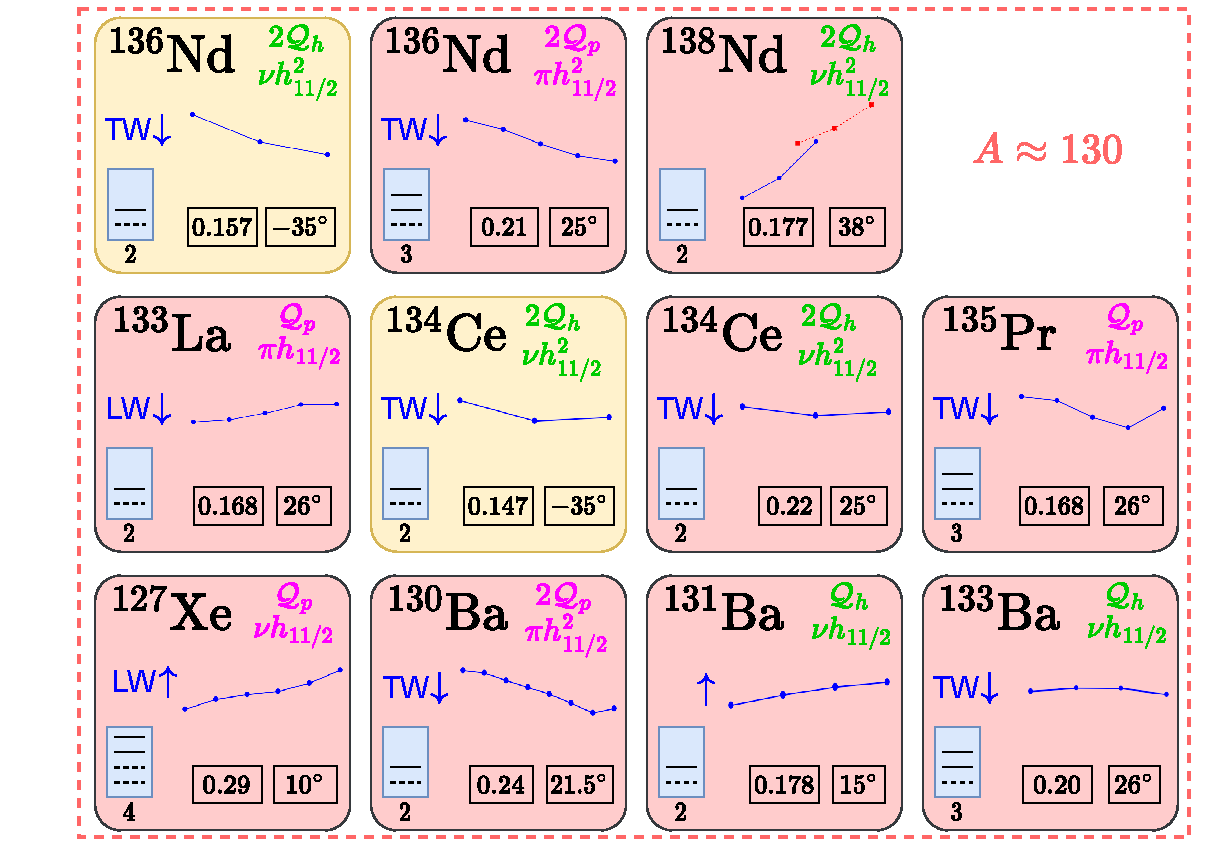
\includegraphics[width=0.87\textwidth]{figures/wobblers-chart-2.pdf}
	\end{figure}
\end{frame}

\begin{frame}
	\frametitle{Wobblers in the A=160 mass region}
	\begin{figure}
		\centering
		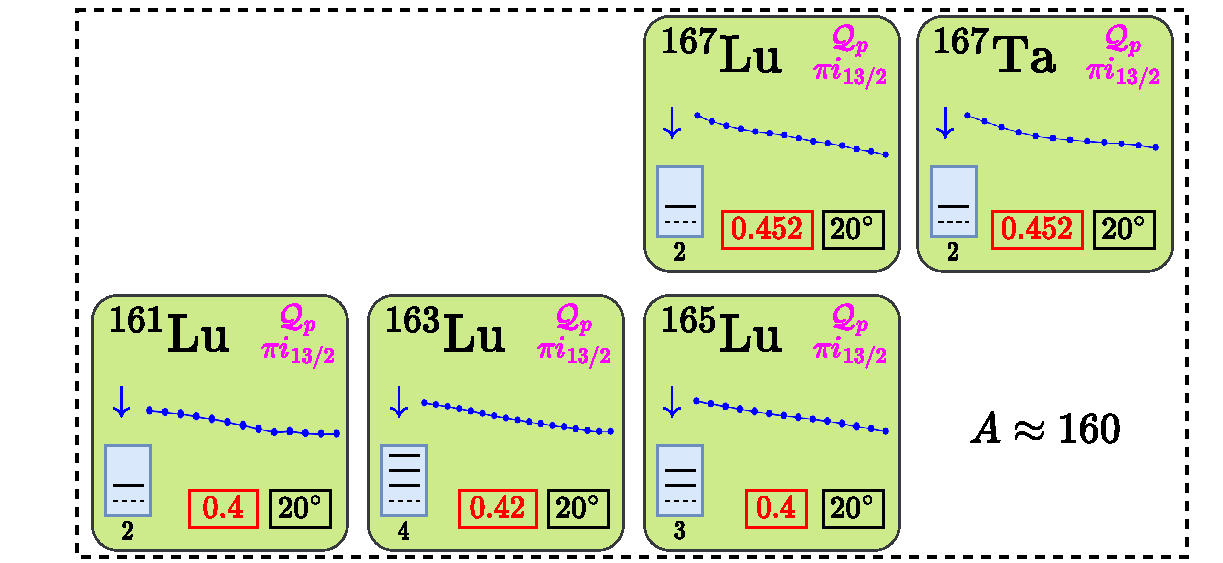
\includegraphics[width=0.99\textwidth]{figures/wobblers-chart-4.pdf}
	\end{figure}
\end{frame}

\begin{frame}
	\frametitle{Wobblers in the A=180 mass region}
	\begin{figure}
		\centering
		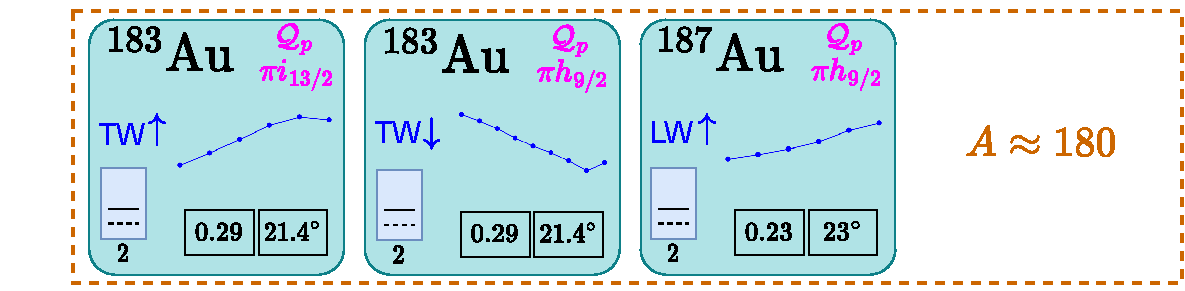
\includegraphics[width=0.99\textwidth]{figures/wobblers-chart-3.pdf}
	\end{figure}
	% \begin{figure}
	% 	\centering
	% 	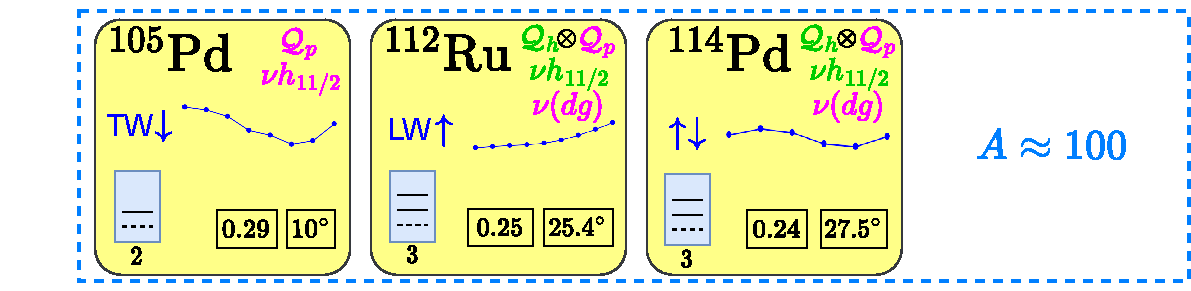
\includegraphics[width=0.99\textwidth]{figures/wobblers-chart-1.pdf}
	% \end{figure}
	\begin{beamercolorbox}[rounded=true,shadow=false, wd=\linewidth,]{block body}
		\centering
		\textcolor{black}{All diagrams and their data sources available in Chapter 3, Section 3.3.5}\\
		\textcolor{red}{\textbf{Presented at the Annual Meeting, FFUB, 2022.}}
	\end{beamercolorbox}
\end{frame}

\subsection{Even-A case study}

\begin{frame}
	\frametitle{Wobbling Motion in $^{130}$Ba}
	\begin{columns}
		\begin{column}{0.55\textwidth}
			\faSearch\ Experimental measurements show \textbf{two} wobbling bands (\textit{Petrache et. al. 2019}).
			\begin{exampleblock}{Harmonic formalism}
				\textbf{Harmonic Approximation} (\textit{Bohr \& Mottelson, 1969}):
				\begin{align}
					E_{I,n_w}&={\color{red}A_3I(I+1)}+{\color{blue}\hbar\omega_w\left(n_w+\frac{1}{2}\right)}\nonumber,\\
					A_3&=(2\mathcal{I}_3)^{-1}\nonumber.
				\end{align}
				({\color{red}rotational term} + {\color{blue}wobbling frequency})
			\end{exampleblock}
		\end{column}
		\begin{column}{0.45\textwidth}
			\begin{figure}
				\centering
				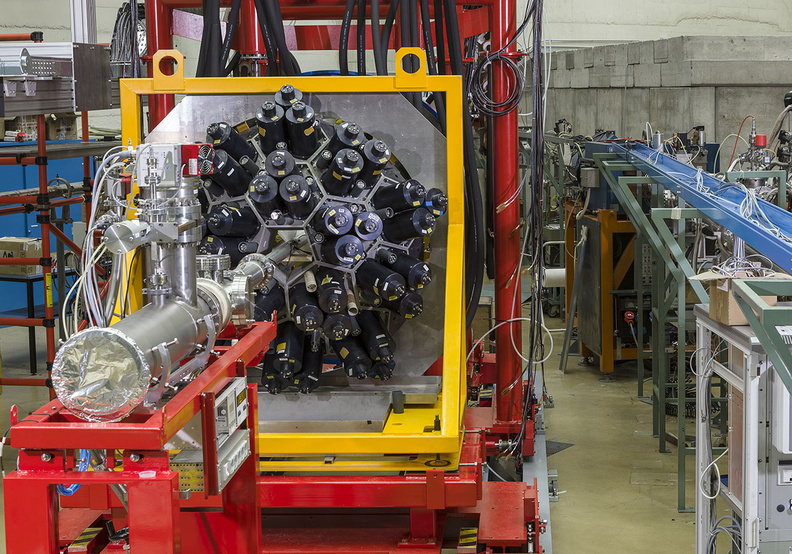
\includegraphics[width=0.99\textwidth]{figures/galileo_exp.jpg}
				{\footnotesize GALILEO, LNL, \textit{Source: lnl.infn.it}}
			\end{figure}
			{\footnotesize Fusion evaporation: $^{13}$C beam of $E=65\ \text{MeV}$ and $^{122}$Sn target.}
		\end{column}
	\end{columns}
\end{frame}

\begin{frame}
	\frametitle{Results for $^{130}$Ba}
	\begin{columns}
		\begin{column}{0.6\textwidth}
			\begin{figure}
				\centering
				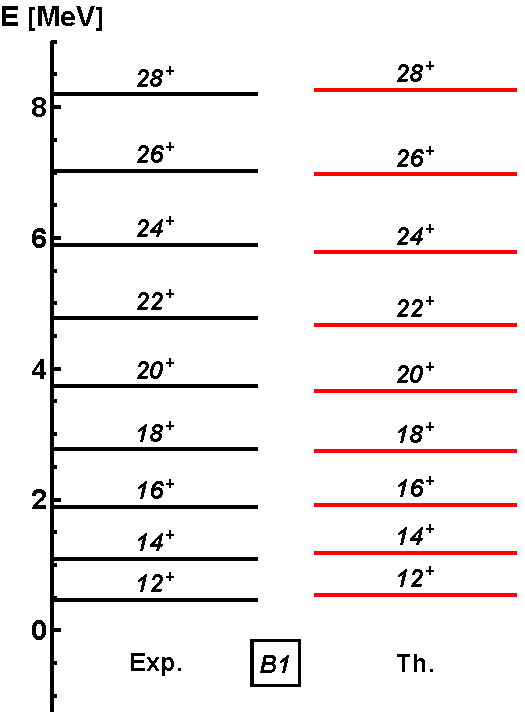
\includegraphics[width=0.49\textwidth]{figures/ba130-band1.pdf}
				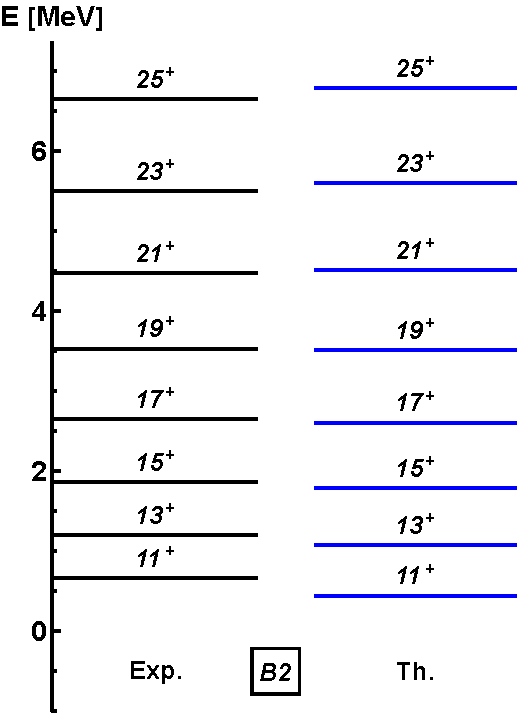
\includegraphics[width=0.49\textwidth]{figures/ba130-band2.pdf}
			\end{figure}				
		\end{column}
		\begin{column}{0.4\textwidth}
			\begin{table}
				\centering
				% \caption{The parameter set obtained from the \emph{fitting procedure}.}
				\resizebox{0.9\textwidth}{!}{%
				\begin{tabular}{cccc}
				\hline
				\multicolumn{4}{c}{$\mathcal{P}_\text{fit}$} \\ \hline \hline
				\multicolumn{1}{c}{$\mathcal{I}_1$} & \multicolumn{1}{c}{$\mathcal{I}_2$} & \multicolumn{1}{c}{$\mathcal{I}_3$} & \multicolumn{1}{c}{Unit}                     \\ \hline
				\multicolumn{1}{c}{27}              & \multicolumn{1}{c}{22}              & \multicolumn{1}{c}{\textbf{43}}              & \multicolumn{1}{c}{$\hbar^2\text{MeV}^{-1}$} \\ \hline
				\end{tabular}%
				}
				\label{table-params-ba130}
			\end{table}
			\begin{figure}
				\centering
				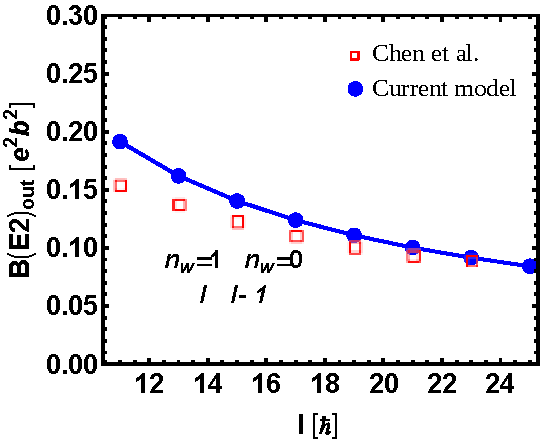
\includegraphics[width=0.99\textwidth]{figures/ba130-EM.pdf}
			\end{figure}
		\end{column}
	\end{columns}
	
	% use color box
	% \begin{tcolorbox}[colback=white, colframe=black, arc=2mm]
		% 	\centering
		% 	\begin{beamercolorbox}[rounded=true,shadow=false, wd=\linewidth,]{block body}
			% 		\centering
			% 		\textcolor{red}{\textit{Results presented at the international conference NSP, 2022, Turkey.}}
			% 	\end{beamercolorbox}
			% \end{tcolorbox}
			
	% no color box
	\begin{beamercolorbox}[rounded=true,shadow=false, wd=\linewidth,]{block body}
		\centering
		Full description: Chapter 3 (Section 3.1.2)\\
		\textcolor{red}{\textbf{Results presented at the international conference NSP-2022, Turkey.}}
	\end{beamercolorbox}
\end{frame}

\begin{frame}
	\frametitle{Results for $^{130}$Ba II}
	\textbf{Excitation energies} vs. \textbf{Wobbling Energies}:
	\begin{align}
		E_\text{wob}(I_\text{even})&=E_{I,n}-E_{I,0}\ ,\nonumber \\
		E_\text{wob}(I_\text{odd})&=E_{I,n}-\frac{1}{2}\left(E_{I-1,0}+E_{I+1,0}\right) \nonumber
	\end{align}
	\vspace{-0.6cm}
	\begin{figure}
		\centering
		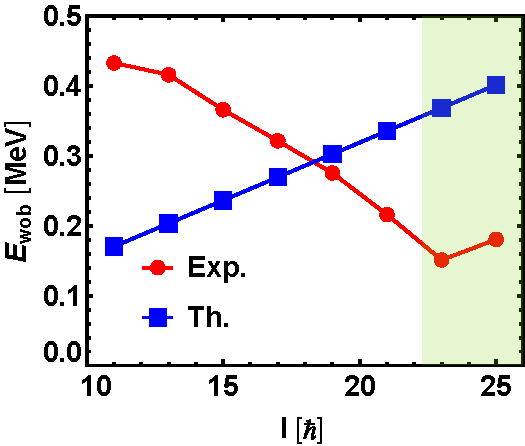
\includegraphics[scale=0.6]{figures/ba130-wobbling-energies-edited.pdf}
		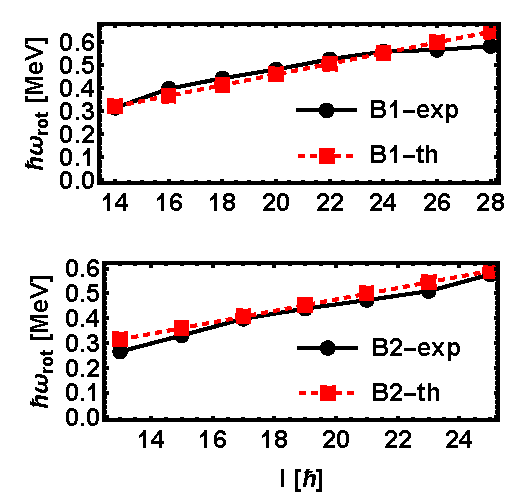
\includegraphics[scale=0.55]{figures/ba130-rotational-frequencies.pdf}
	\end{figure}
	\vspace{-0.2cm}
	\begin{beamercolorbox}[rounded=true,shadow=false, wd=\linewidth,]{block body}
		\centering
		\textcolor{red}{\small{\textbf{Results presented at the international conference NSP-2022, Turkey.}}}
	\end{beamercolorbox}
\end{frame}

\section{Wobbling Motion in Odd-A}

\subsection{Old formalism}

\begin{frame}
	\frametitle{Starting Point}
	\begin{columns}
		\begin{column}{0.6\textwidth}
			{\footnotesize \faFile\ A. A. Raduta, \textbf{R. Poenaru}, L. Gr. Ixaru, PRC, 2017} + {\footnotesize \faFile\ A. A. Raduta, \textbf{R. Poenaru}, Al. H. Raduta, JPG, 2018}$\to${\footnotesize $\mathbf{W}_0$ in the thesis.}
			\begin{exampleblock}{Framework}
				\begin{itemize}
					\item \textbf{First semi-classical description} for the $^{163}$Lu, using the \textbf{Particle-Rotor-Model} (\textit{Hamamoto, 2002}.) for an odd-mass nucleus in the $A\approx 160$ region.
				\end{itemize}
			\end{exampleblock}
			\begin{alertblock}{PRM}
				\textbf{An odd-nucleon moving in a quadrupole deformed mean field generated by an even-even triaxial core.}
			\end{alertblock}
		\end{column}
		\begin{column}{0.4\textwidth}
			\begin{figure}
				\centering
				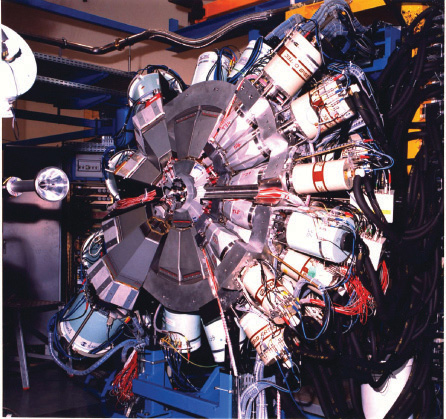
\includegraphics[width=0.99\textwidth]{figures/euroball-4.jpg}
				{\footnotesize Euroball IV, Strasbourg, \textit{Source: technologysi.stfc.ac.uk}}
			\end{figure}
			{\footnotesize Fusion evaporation: $^{29}$Si beam of $E=152\ \text{MeV}$ and $^{139}$La target.}
		\end{column}
	\end{columns}
\end{frame}

\begin{frame}
	\frametitle{Overview of $\mathbf{W}_0$}
	\vspace{-0.3cm}
	\begin{columns}
		\begin{column}{0.6\textwidth}
			\begin{itemize}
				\item Time-Dependent Variational Principle applied on the PRM Hamiltonian
				\item \textbf{Phonon operators} $\rightarrow$ energies + transition probabilities
			\end{itemize}
			\vspace{-0.5cm}
			\begin{figure}
				\centering
				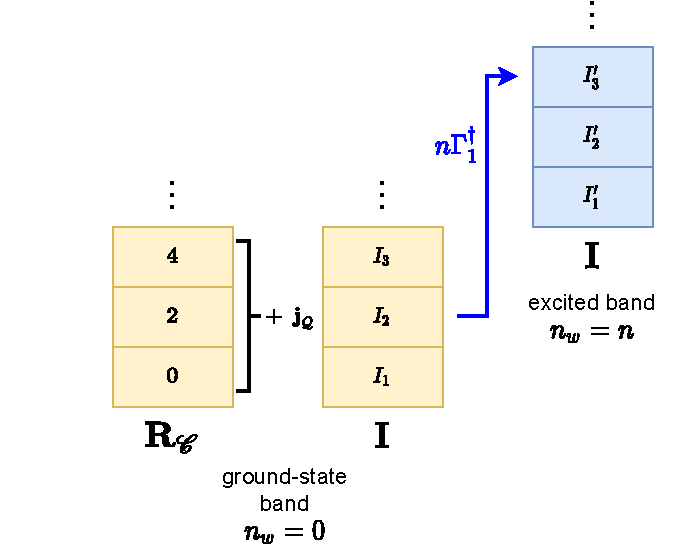
\includegraphics[width=0.9\textwidth]{figures/w0_phonon_operator.pdf}
			\end{figure}
		\end{column}
		\begin{column}{0.4\textwidth}
			\begin{figure}
				\centering
				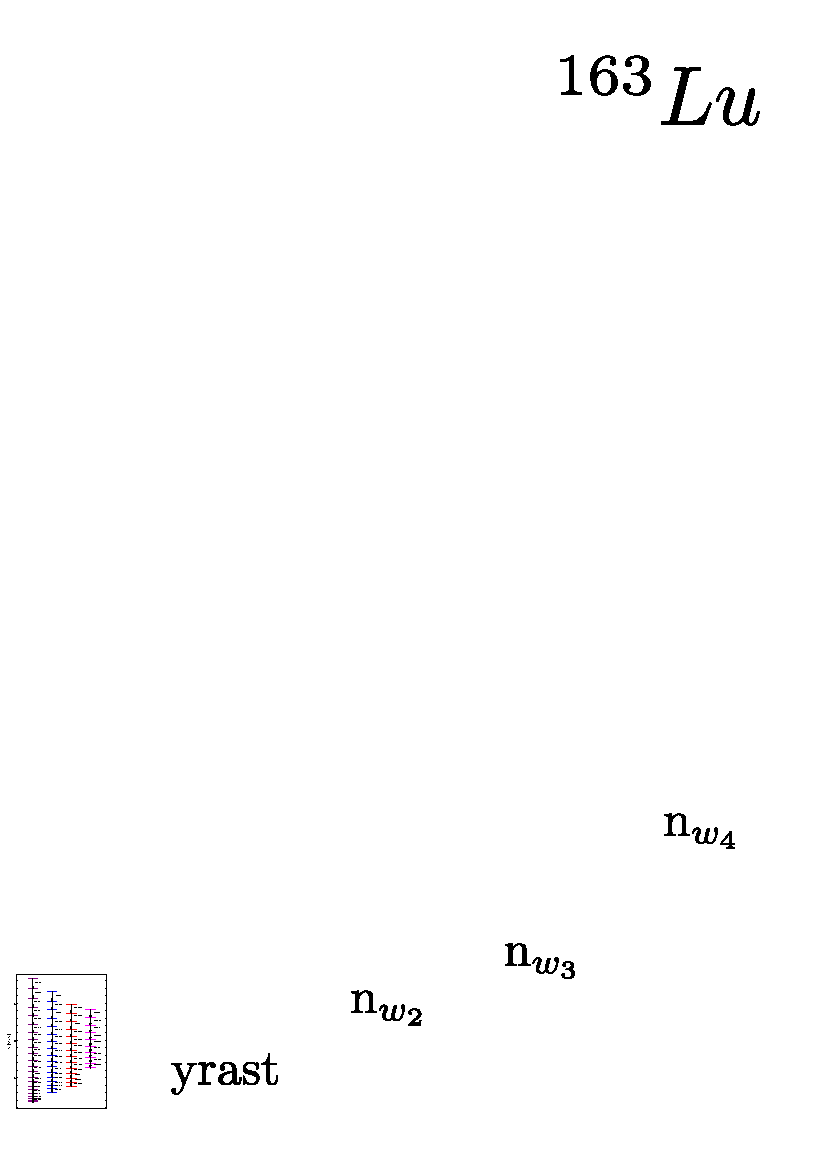
\includegraphics[width=0.99\textwidth]{figures/lu-163-exp-data.eps}
			\end{figure}
		\end{column}
	\end{columns}
\end{frame}


\begin{frame}
	\frametitle{Overview of $\mathbf{W}_0$ II}
	\begin{block}{Model characteristics}
		\faPlus\ Numerical data consistent with other work\\
		\faMinus\ TSD4: three-phonon wobbling band (disagreement with Jensen et al.)\\
		\faMinus\ Adopted rigid-body MOIs ("unpleasant" choice to the referees) \\
		\faMinus\ Deformation parameters $\beta$ and $\gamma$ taken from literature
	\end{block}
	\vspace{0.4cm}
	\begin{beamercolorbox}[rounded=true,shadow=false, wd=\linewidth,]{block body}
		\centering
		\textcolor{black}{\small{\textbf{Onset of a redesign $\longrightarrow$ start of a new research project}}}\\
		\textcolor{black}{\small{\textbf{Two new models developed presented in Chapter 4 ($\mathbf{W}_1$) and 5 ($\mathbf{W}_2$)}}}\\
	\end{beamercolorbox}
\end{frame}
\subsection{Redefinition of the Odd-A framework}

\begin{frame}
	\frametitle{Fresh-up: $\mathbf{W}_1$}
	Particle-Rotor Model Hamiltonian for an odd-$A$ nucleus:	
	% \begin{align}
	% 	\hat{H}={\color{red}\hat{H}_\text{rot}}+{\color{blue}\hat{H}_\text{sp}}\nonumber\\
	% 	{\color{red}\hat{H}_\text{rot}}={\color{red}\sum_{k=1}^3A_k(\hat{I}_k-\hat{j}_k)^2}\nonumber\\
	% 	{\color{blue}\hat{H}_\text{sp}}={\color{blue}\epsilon_j+\frac{V}{j(j+1)}\left[\cos\gamma\left(3\hat{j}_3^3-\mathbf{j}_\mathcal{Q}^2\right)-\sqrt{3}\sin\gamma\left(\hat{j}_1^2-\hat{j}_2^2\right)\right]}\nonumber
	% \end{align}
	\begin{alignat*}{2}
		\hat{H}&={\color{red}\hat{H}_\text{rot}}+{\color{blue}\hat{H}_\text{sp}}\ ,\ {\color{red}\hat{H}_\text{rot}}={\color{red}\sum_{k=1}^3A_k(\hat{I}_k-\hat{j}_k)^2},\\
		{\color{blue}\hat{H}_\text{sp}}&={\color{blue}\epsilon_j+\frac{V}{j(j+1)}\left[\cos\gamma\left(3\hat{j}_3^3-\mathbf{j}^2\right)-\sqrt{3}\sin\gamma\left(\hat{j}_1^2-\hat{j}_2^2\right)\right]}
	\end{alignat*}
	\vspace{-0.4cm}
	\begin{figure}
		\centering
		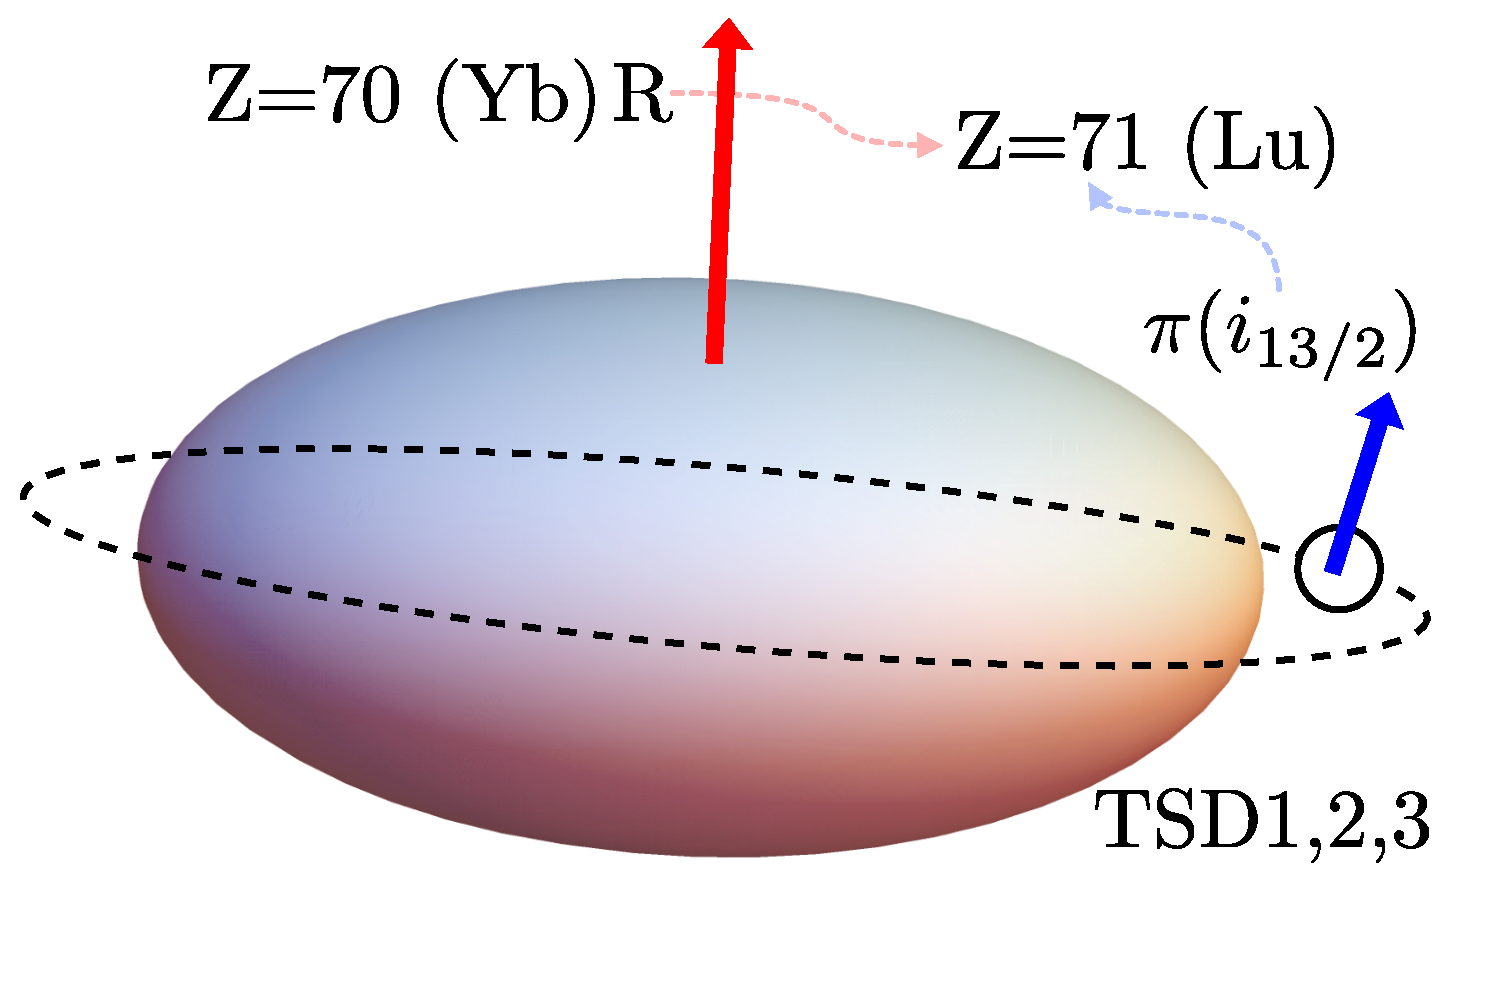
\includegraphics[scale=0.22]{figures/triaxial-shapes-oddA-1.pdf}
		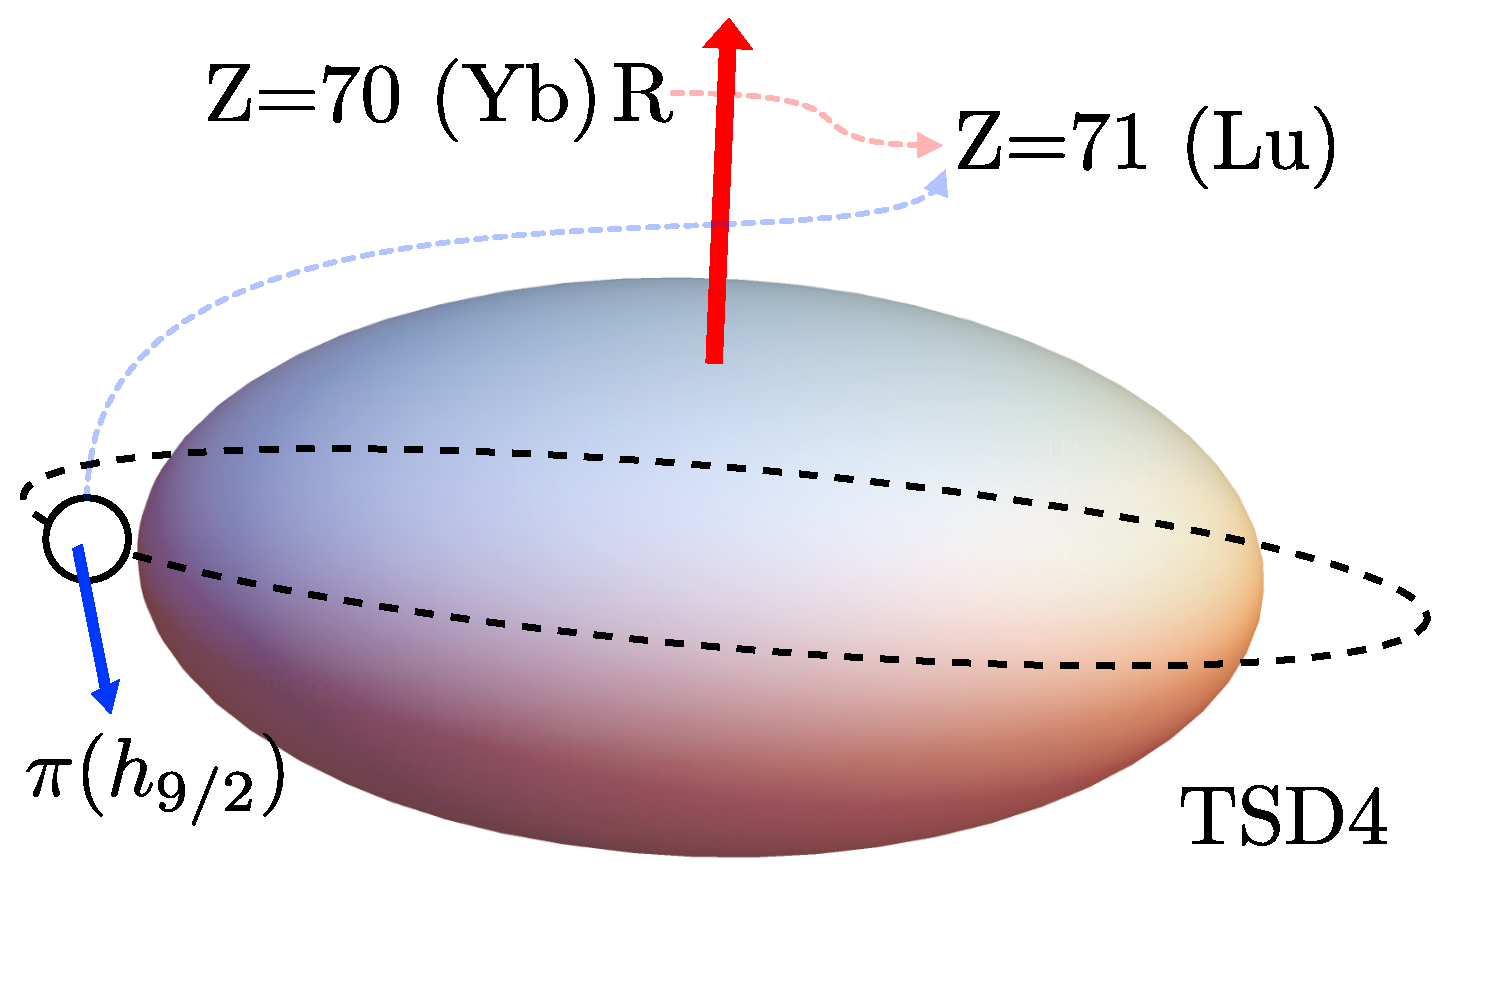
\includegraphics[scale=0.22]{figures/triaxial-shapes-oddA-2.pdf}
	\end{figure}
	\vspace{-0.5cm}
	\begin{beamercolorbox}[rounded=true,shadow=false, wd=\linewidth,]{block body}
		\centering
		\textcolor{red}{\footnotesize{A. A. Raduta, \textbf{R. Poenaru}, C. M. Raduta, Phys. Rev. C 101, 2020.}}
	\end{beamercolorbox}
\end{frame}

\begin{frame}
	\frametitle{Variational Principle + Eqs. of Motion}
	\begin{columns}
		\begin{column}{0.6\textwidth}
			\begin{exampleblock}{Time-Dependent Varational Equation}
				\begin{align}
					\delta&\int_0^t\bra{\Psi_{IM;j}}\hat{H}-i\frac{\partial}{\partial t'}\ket{\Psi_{IM;j}}dt'=0\nonumber\\
					\Psi_\text{trial}&\equiv\ket{\Psi_{IM;j}}=\mathcal{N}{\color{red}e^{z\hat{I}_-}}\cdot{\color{blue}e^{s\hat{j}_-}}{\color{red}\ket{IMI}}\otimes{\color{blue}\ket{jj}}\nonumber
				\end{align}
				\vspace{-0.4cm}
				\begin{itemize}
					\item {\color{red}$(z,r,\varphi,\hat{I},\ket{IMI})$} - core ({\color{red}$\mathbf{R}$})
					\item {\color{blue}$(s,f,\psi,\hat{j},\ket{jj})$} - single-particle ({\color{blue}$\mathbf{j}$})
					\item {\color{blue}$(s,f,\psi,\hat{j},\ket{jj})$} - single-particle ({\color{blue}$\mathbf{j}$})
					\item $\{z,s\}\ \rightarrow$ \textbf{phase space coordinates}
				\end{itemize}
			\end{exampleblock}
		\end{column}
		\begin{column}{0.4\textwidth}
			\textbf{Constant of motion:}
			\begin{align}
				\mathcal{H}\equiv\bra{\Psi_{IM;j}}\hat{H}\ket{\Psi_{IM;j}}\nonumber
			\end{align}
			\textbf{Canonical equations of motion:}
			\begin{align}
				{\color{red}\mathcal{S}_1: \frac{\partial \mathcal{H}}{\partial r}=\dot{\varphi}\ ,\ \frac{\partial \mathcal{H}}{\partial \varphi}=-\dot{r}}\nonumber\\
				{\color{blue}\mathcal{S}_2: \frac{\partial \mathcal{H}}{\partial f}=\dot{\psi}\ ,\ \frac{\partial \mathcal{H}}{\partial \psi}=-\dot{f}}\nonumber
			\end{align}
		\end{column}
	\end{columns}
	\begin{beamercolorbox}[rounded=true,shadow=false, wd=\linewidth,]{block body}
		\centering
		\textcolor{black}{\small{The two sets of Hamilton equations are \textbf{the semi-classical description} of the initial quantal $\hat{H}$.}}
	\end{beamercolorbox}
\end{frame}


\begin{frame}
	\frametitle{Wobbling frequency}
	Solving {\color{red}$\mathcal{S}_1$} and {\color{blue}$\mathcal{S}_2$} leads to the algebraic equation:
	\begin{align}
		\Omega^4+B\Omega^2+C=0\nonumber
	\end{align}
	four solutions $\longrightarrow$ \textbf{only two are real}:
	\begin{align}
		\Omega_{1,2}=\left[\frac{1}{2}\left(-B\mp\sqrt{B^2-4C}\right)\right]^{1/2}\nonumber
	\end{align}
	\vspace{-0.3cm}
	\begin{beamercolorbox}[rounded=true,shadow=false, wd=\linewidth,]{block body}
		\centering
		\textcolor{red}{\footnotesize{A. A. Raduta, \textbf{R. Poenaru}, C. M. Raduta, Phys. Rev. C 101, 2020.}}
	\end{beamercolorbox}
	\vspace{-0.3cm}
	\begin{itemize}
		\item {\color{red}$\Omega_1$}: wobbling frequency of the {\color{red}even-$A$ core $\mathbf{R}$}
		\item {\color{blue}$\Omega_2$}: wobbling frequency of the {\color{blue}odd-nucleon $\mathbf{j}$}
		\item \textbf{Two wobbling phonon numbers: {\color{red}$n_{w_1}$} and {\color{blue}$n_{w_2}$}}
	\end{itemize}
\end{frame}

\begin{frame}
	\frametitle{Energy spectrum}
	\begin{exampleblock}{Spectra of odd-A nuclei within $\mathbf{W}_1$}
		\begin{align}
			E_{I,n_1,n_2}=\epsilon_j+\mathcal{H}_\text{min}^I+\hbar\Omega_1^I\left(n_{w_1}+\frac{1}{2}\right)+\hbar\Omega_2^I\left(n_{w_2}+\frac{1}{2}\right)\nonumber
			\label{tsd-bands-general-spectrum}
		\end{align}
	\end{exampleblock}
	\begin{itemize}
		\item Phonon factor:
		\begin{align}
			\mathcal{F}_{n_{w_1}n_{w_2}}^I&=\hbar\Omega_1^I\left(n_{w_1}+\frac{1}{2}\right)+\hbar\Omega_2^I\left(n_{w_2}+\frac{1}{2}\right)\nonumber
		\end{align}
		\item $\mathcal{H}_\text{min}^I$ is the Classical Energy Function taken in its minimum point: $p_0=(0,I;0,j)$.
	\end{itemize}
\end{frame}

\begin{frame}
	\frametitle{A new interpretation for TSD1 and TSD2}
	\begin{exampleblock}{Previous models}
		$TSD1=$ zero-phonon wobbling band\\
		$TSD2=$ one-phonon wobbling band...
	\end{exampleblock}
	\begin{alertblock}{Redefinition}
		$TSD1$ and $TSD2$ are \textbf{Signature Partner Bands} (In favor of Ultimate Cranker calculations, \textit{Jensen, 2004}).
		\begin{align}
			\left(\alpha_{fav}=+\frac{1}{2}\right): \{TSD1\}&\equiv\left\{\left[0^+,2^+,4^+,\dots\right] \otimes [j^\pi=13/2^+]\right\}\nonumber\\
			\left(\alpha_{unfav}=-\frac{1}{2}\right): \{TSD2\}&\equiv\left\{\left[1^+,3^+,5^+,\dots\right] \otimes [j^\pi=13/2^+]\right\}\nonumber
		\end{align}
		$TSD4$: \textbf{ground-state wobbling band}, $\pi(h_{9/2})$ configuration.
	\end{alertblock}
	\begin{beamercolorbox}[rounded=true,shadow=false, wd=\linewidth,]{block body}
		\centering
		\textcolor{red}{\footnotesize{A. A. Raduta, \textbf{R. Poenaru}, C. M. Raduta, Phys. Rev. C 101, 2020.}}
	\end{beamercolorbox}
\end{frame}

\begin{frame}
	\frametitle{A new band structure for $^{163}$Lu}
	\begin{table}
		\centering
		\resizebox{\textwidth}{!}{%
		\begin{tabular}{ccccccc}
		\hline
		Band & Spins & $\pi$ & $\alpha$ & $\pi(l_j)$ & $\mathbf{W_0}$: $\mathscr{C}+\mathcal{Q}_p$ & $\mathbf{W_1}$: $\mathscr{C}+\mathcal{Q}_p$ \\ \hline \hline
		TSD1 & $13/2,17/2 \dots 97/2$ & $+$ & $+1/2$ & $\pi(i_{13/2})$ & $0^+,2^+,4^+,\dots$ & $0^+,2^+,4^+,\dots$ \\ \hline
		TSD2 & $27/2,31/2 \dots 91/2$ & $+$ & $-1/2$ & $\pi(i_{13/2})$ & $\text{TSD1}+1\Gamma^\dagger$ & $1^+,3^+,5^+,\dots$ \\ \hline
		TSD3 & $33/2,37/2 \dots 85/2$ & $+$ & $+1/2$ & $\pi(i_{13/2})$ & $\text{TSD1}+2\Gamma^\dagger$ & $\text{TSD2}+\Gamma^\dagger$ \\ \hline
		TSD4 & $47/2,51/2 \dots 83/2$ & $-$ & $-1/2$ & $\pi(h_{9/2})$  & $\text{TSD1}+3\Gamma^\dagger$ & $1^+,3^+,5^+,\dots$ \\ \hline
		\end{tabular}%
		}
	\end{table}
	\begin{table}
		\centering
		\resizebox{\textwidth}{!}{%
		\begin{tabular}{ccccccc}
		\hline
		Bands & $n_{w_1}$ & $n_{w_2}$ & $\mathcal{F}_{n_{w_1}n_{w_2}}^I$ & $I_0$    & $I_t$    & $\mathcal{Q}$    \\ \hline \hline 
		TSD1  & $0$       & $0$       & $\mathcal{F}_{00}^I=\frac{1}{2}\left(\Omega_1^I+\Omega_2^I\right)$ & $13/2^+$ & $97/2^+$ & $j^\pi=13/2^+\stackrel{not}{\equiv}\mathcal{Q}_1$ \\ \hline
		TSD2  & $\mathbf{0}$       & $\mathbf{0}$       & $\mathcal{F}_{00}^I=\frac{1}{2}\left(\Omega_1^I+\Omega_2^I\right)$ & $27/2^+$ & $91/2^+$ & $j^\pi=13/2^+\stackrel{not}{\equiv}\mathcal{Q}_1$ \\ \hline
		TSD3  & $1$       & $0$       & $\mathcal{F}_{10}^{I-1}=\frac{3}{2}\Omega_1^{I-1}+\frac{1}{2}\Omega_2^{I-1}$ & $33/2^+$ & $85/2^+$ & $j^\pi=13/2^+\stackrel{not}{\equiv}\mathcal{Q}_1$ \\ \hline
		\textbf{TSD4}  & $\mathbf{0}$       & $\mathbf{0}$       & $\mathcal{F}_{00}^I=\frac{1}{2}\left(\Omega_1^I+\Omega_2^I\right)$ & $47/2^-$ & $83/2^-$ & $j^\pi=9/2^-\stackrel{not}{\equiv}\mathcal{Q}_2$  \\ \hline
		\end{tabular}%
		}
	\end{table}
	\vspace{-0.3cm}
	\begin{beamercolorbox}[rounded=true,shadow=false, wd=\linewidth,]{block body}
		\centering
		\textcolor{red}{\footnotesize{A.A. Raduta, \textbf{R. Poenaru}, C.M. Raduta, Journal of Physics G 47, 2020.}}
	\end{beamercolorbox}
\end{frame}

\begin{frame}
	\frametitle{Extension to $A\approx160$ mass region}
	\vspace{-0.5cm}
	The model was further applied to the other Lu isotopes where wobbling motion has been observed.
	\vspace{-0.5cm}
	\begin{table}
		\centering
		\resizebox{\textwidth}{!}{%
		\begin{tabular}{cccccc}
			\hline
			$^{161}$Lu Bands & Spins                        & $\mathcal{Q}$ & $\mathscr{C}$  & $(n_{w_1},n_{w_2})$ & $I_b$                   \\ \hline \hline
			TSD1 & $21/2^+,25/2^+,\dots,89/2^+$ & $j^\pi=13/2^+$  & $4^+,6^+,8^+\dots$   & $(0,0)$             & \multirow{2}{*}{$21/2$} \\ \cline{1-5}
			TSD2 & $31/2^+,35/2^+,\dots,79/2^+$ & $j^\pi=13/2^+$  & $9^+,11^+,13^+\dots$ & $(0,0)$             &                         \\ \hline
		\end{tabular}%
		}
		\label{lu-161-experimental-data-table}
	\end{table}
	\vspace{-0.5cm}
	\begin{table}
		\centering
		\resizebox{\textwidth}{!}{%
		\begin{tabular}{cccccc}
			\hline
			$^{165}$Lu Bands & Spins                        & $\mathcal{Q}$ & $\mathscr{C}$         & $(n_{w_1},n_{w_2})$ & $I_b$                   \\ \hline \hline
			TSD1 & $25/2^+,29/2^+,\dots,89/2^+$ & $j^\pi=13/2^+$  & $6^+,8^+,10^+\dots$   & $(0,0)$             & \multirow{3}{*}{$25/2$} \\ \cline{1-5}
			TSD2 & $35/2^+,39/2^+,\dots,91/2^+$ & $j^\pi=13/2^+$  & $11^+,13^+,15^+\dots$ & $(0,0)$             &                         \\ \cline{1-5}
			TSD3 & $41/2^+,45/2^+,\dots,81/2^+$ & $j^\pi=13/2^+$  & $\text{TSD2}+\Gamma^\dagger$ & $(1,0)$             &                         \\ \hline
		\end{tabular}%
		}
		\label{lu-165-experimental-data-table}
	\end{table}
	\vspace{-0.5cm}
	\begin{table}
		\centering
		\resizebox{\textwidth}{!}{%
		\begin{tabular}{cccccc}
			\hline
			$^{167}$Lu Bands & Spins                        & $\mathcal{Q}$ & $\mathscr{C}$         & $(n_{w_1},n_{w_2})$ & $I_b$                   \\ \hline \hline
			TSD1 & $25/2^+,29/2^+,\dots,89/2^+$ & $j^\pi=13/2^+$  & $6^+,8^+,10^+\dots$   & $(0,0)$             & \multirow{2}{*}{$25/2$} \\ \cline{1-5}
			TSD2 & $35/2^+,39/2^+,\dots,91/2^+$ & $j^\pi=13/2^+$  & $11^+,13^+,15^+\dots$ & $(0,0)$             &                         \\ \hline
		\end{tabular}%
		}
		\label{lu-167-experimental-data-table}
	\end{table}
	\begin{beamercolorbox}[rounded=true,shadow=false, wd=\linewidth,]{block body}
		\centering
		\textcolor{red}{\footnotesize{A. A. Raduta, \textbf{R. Poenaru}, C. M. Raduta, Phys. Rev. C 101, 2020.}}
	\end{beamercolorbox}
\end{frame}

\begin{frame}
	\frametitle{$\mathbf{W}_1$ | Numerical Results}
\end{frame}

% \item Predicted: more than 50 years ago. First confirmed for $^{163}$Lu (\textit{Ødegård} et. al., 2001)
% \item Currently confirmed wobblers $A\approx[100,130,160,180]$.


% \begin{frame}
%     \transduration<0-5>{0}
%     \multiinclude[<+->][format=png, graphics={width=\textwidth}]{figures/wobbler-gif/wobbler}
%     % \animategraphics[loop,controls,width=\linewidth]{10}{figures/wobbler-gif/wobbler-}{0}{5}
% \end{frame}

\begin{frame}[plain] % The optional argument 'plain' hides the headline and footline
	\begin{center}
		\bigskip\bigskip % Vertical whitespace
		{\Huge Thank you for your attention \faHeart}
	\end{center}
\end{frame}

\end{document}
